\documentclass[varwidth]{standalone}

\usepackage{tikzlings}

\newcommand{\foo}{%
%hat%
%strawhat%
%harlequin%
%witch%
%queencrown%
%kingcrown%
%santa%
%graduate%
%alien%
%book%
%pizza%
%baguette%
%cake%
%icecream%
%wine%
%magicwand%
%rollingpin%
%basket%
%crozier%
%shovel%
%pickaxe%
%magichat%
%umbrella%
%umbrellaclosed%
%handbag%
%cocktail%
back%
}

\begin{document}


\begin{tikzpicture}
\bear[\foo]
\end{tikzpicture}\hfill%

\begin{tikzpicture}
\penguin[\foo]
\end{tikzpicture}\hfill%

\begin{tikzpicture}
\marmot[\foo]
\end{tikzpicture}\hfill%

\begin{tikzpicture}
\koala[\foo]
\end{tikzpicture}\hfill%
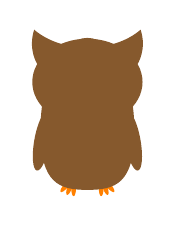
\begin{tikzpicture}
\owl[\foo]
\end{tikzpicture}\hfill%

\begin{tikzpicture}
\coati[\foo]
\end{tikzpicture}


\begin{tikzpicture}
\snowman[\foo]
\end{tikzpicture}\hfill%

\begin{tikzpicture}
\rhino[\foo]
\end{tikzpicture}\hfill%

\begin{tikzpicture}
\moles[\foo]
\end{tikzpicture}\hfill%

\begin{tikzpicture}
\sloth[\foo]
\end{tikzpicture}\hfill%
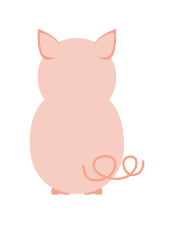
\begin{tikzpicture}
\pig[\foo]
\end{tikzpicture}\hfill%

\begin{tikzpicture}
\cat[\foo]
\end{tikzpicture}


\begin{tikzpicture}
\hippo[\foo]
\end{tikzpicture}\hfill%

\begin{tikzpicture}
\panda[\foo]
\end{tikzpicture}\hfill%

\begin{tikzpicture}
\mouse[\foo]
\end{tikzpicture}

\end{document}
